%%%%%%%%%%%%%%%%%%%%%%%%%%%%%%%%%%%%%%%%%%%%%%%%%%
%
% MPRG Work Document Template
% Copyright (C) 2017 by Tsubasa Hirakawa
%
%%%%%%%%%%%%%%%%%%%%%%%%%%%%%%%%%%%%%%%%%%%%%%%%%%
\RequirePackage[l2tabu, orthodox]{nag}
\documentclass[11pt, a4j]{jarticle}
\usepackage{mprg}
\usepackage{datetime}
\usepackage{ascmac}

%%%%%%%%%%%%%%%%%%%%%%%%%%%%% BODY TEXT %%%%%%%%%%%%%%%%%%%%%%%%%%%%%
\begin{document}


% title %%%%%%%%%%%%%%%%
\title{テンプレート\\
\Large{}}
\author{TP26801 今井　孝洋}
\date{2026年xx月xx日}
\maketitle
\pagestyle{fancy}
%%%%%%%%%%%%%%%%%%%%%%%%


\section{研究テーマ}


\section{主張したいこと}


% \begin{figure}[tb]
% \centering
% 	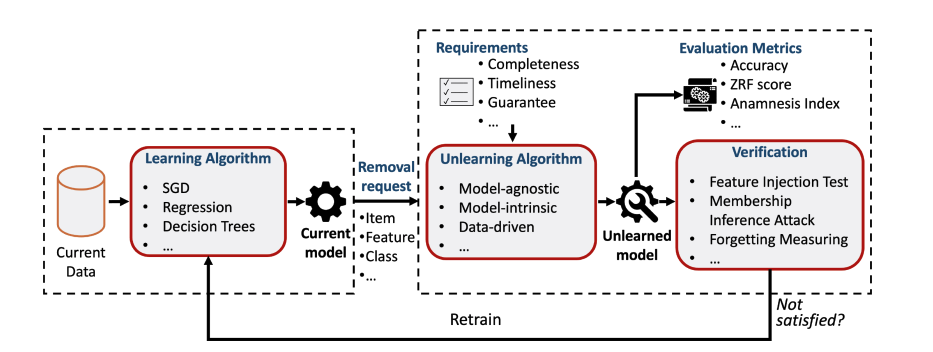
\includegraphics[width=0.95\linewidth]{img/MU/MU_frame.png}
% 	\caption{Machine Unlearningのフレームワーク}
% 	\label{fig:MU_frame}
% \end{figure}





\bibliographystyle{splncs04}
\bibliography{ref}

\end{document} 